\section{Ejercicio 2 - Creación del cubo}  



1. Utilice la base de datos AdventureWorksDW2012 como origen de datos

	\begin{center}
	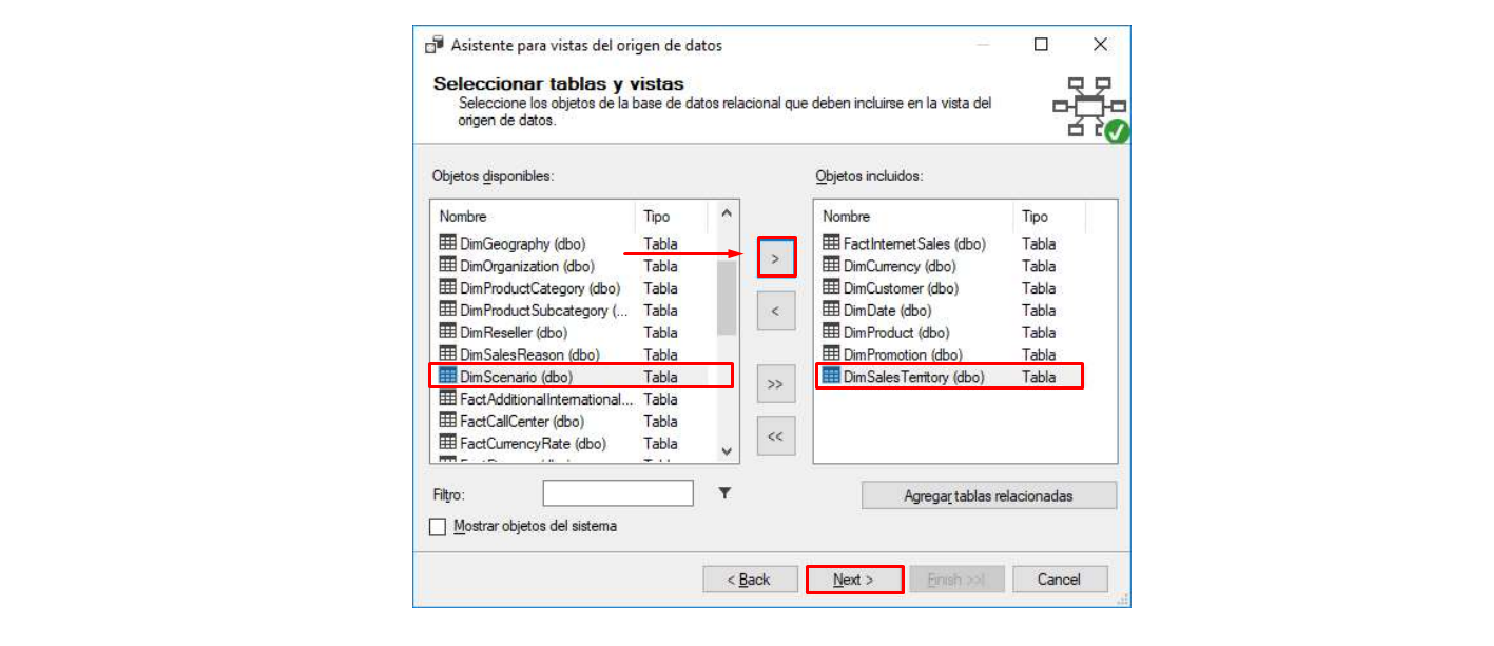
\includegraphics[width=\columnwidth]{images/task2/img1}
	\end{center}	


2. En la opción definir una vista del origen de datos seleccione las siguientes tablas de la base de datos:
FactInternetSales, DimCurrency, DimCustomer, DimDate, DimProduct, DimPromotion, DimSalesTerritory

	\begin{center}
	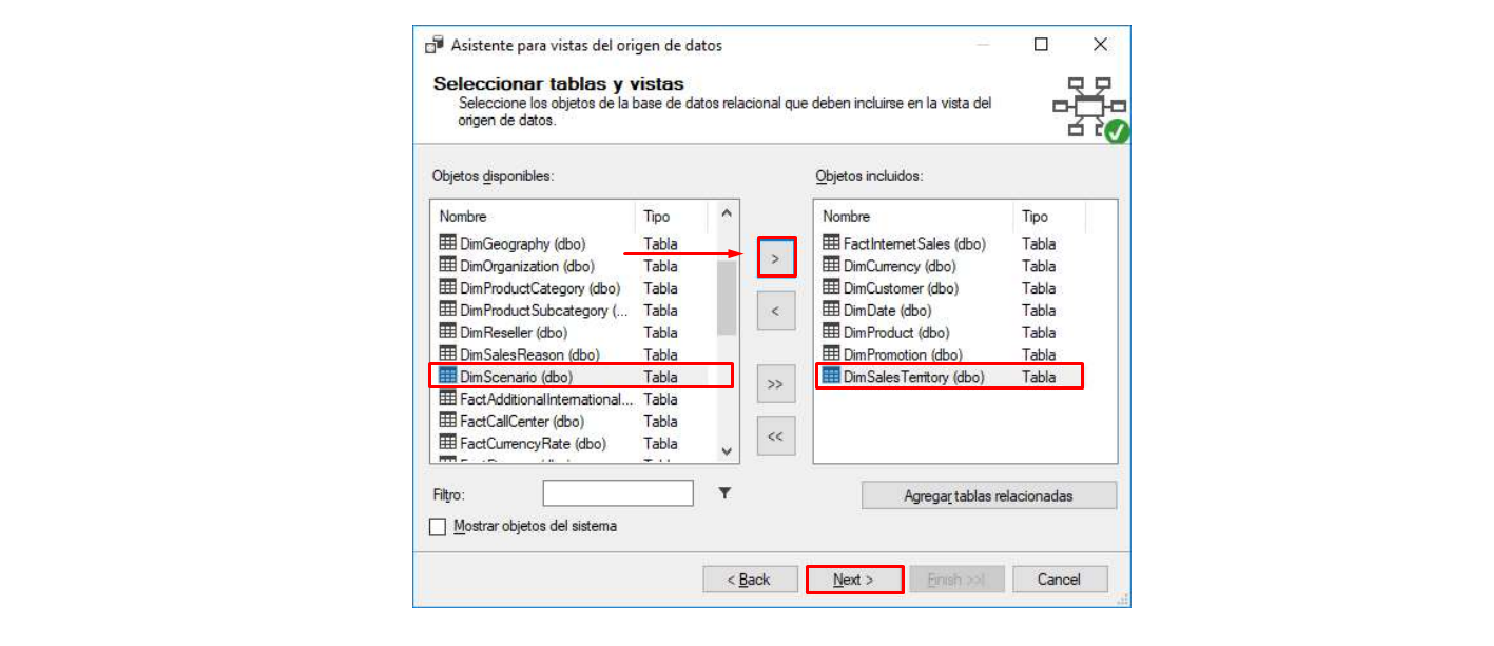
\includegraphics[width=\columnwidth]{images/task2/img2}
	\end{center}	

	\begin{center}
	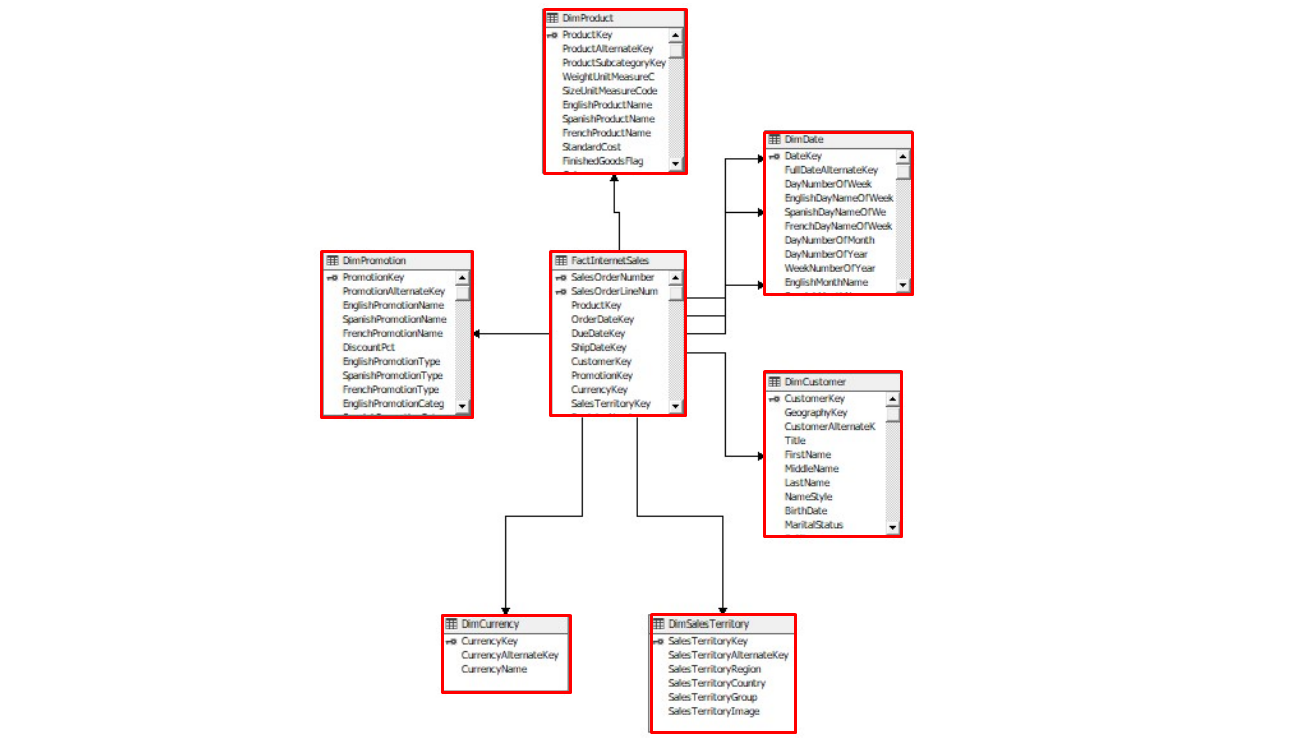
\includegraphics[width=\columnwidth]{images/task2/img3}
	\end{center}	

3. Crear un cubo tomando en cuenta las tablas del origen de datos

	\begin{center}
	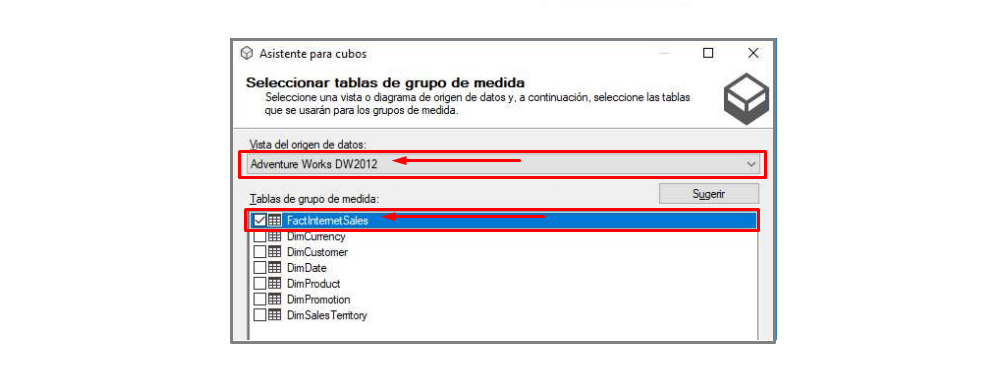
\includegraphics[width=\columnwidth]{images/task2/img4}
    \end{center}	

	\begin{center}
	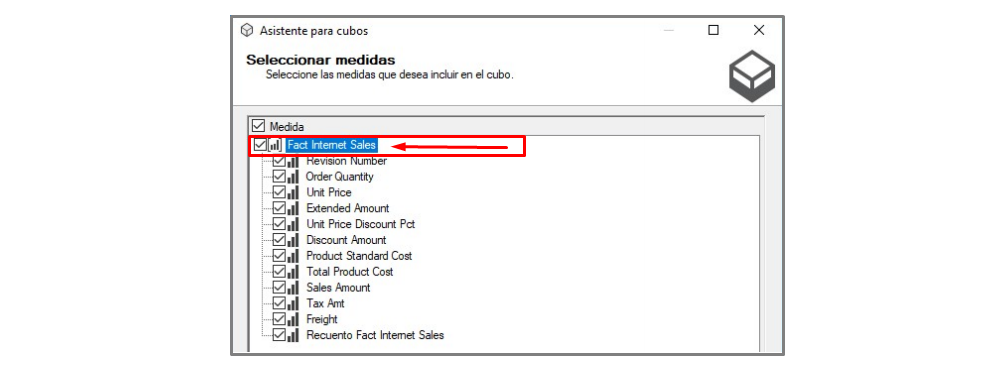
\includegraphics[width=\columnwidth]{images/task2/img5}
    \end{center}	
		
	Procesar el cubo y Examinar el cubo.

4. Cambiar la dimensión Date a:

	\begin{center}
	
\includegraphics[width=\columnwidth]{images/task2/img6}
    \end{center}	



    